% $HeadURL$

\subsection{Glyph: \glyph{Unspecified entity}}
\label{sec:unspecifiedEntity}

The simplest type of EPN is the \glyph{unspecified entity}: one whose type is unknown or simply not relevant to the purposes of the map.  This arises, for example, when the existence of the entity has been inferred indirectly, or when the entity is merely a construct introduced for the needs of a map, without direct biological relevance.  These are examples of situations where the \emph{unspecified entity} glyph is appropriate.  (Conversely, for cases where the identity of the entities composing the pool \emph{is} known, there exist other, more specific glyphs described elsewhere in the specification.)

\begin{glyphDescription}

\glyphSboTerm SBO:0000285 ! material entity of unspecified nature 

\glyphContainer An \glyph{unspecified entity} is represented by an
elliptic container, as shown in \fig{unspecified}.  Note that this
must remain an ellipse to avoid confusion with the Simple Chemical
glyph, which is a circle (c.f.\, \ref{sec:simpleChemical}).

\glyphLabel An \glyph{unspecified entity} is identified by a label
placed in an unbordered box containing a string of characters.  The
characters can be distributed on several lines to improve readability,
although this is not mandatory.  The label box must be attached to the
center of the container.  The label may spill outside of the
container.

\glyphAux An \glyph{unspecified entity} may carry a \glyph{clone marker} (\sect{cloneMarker}).

\end{glyphDescription}

\begin{figure}[H]
  \centering
  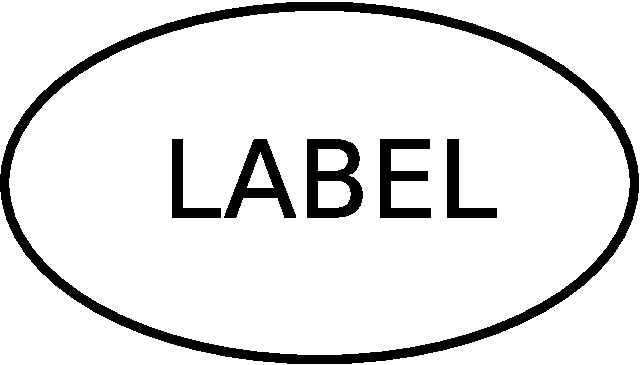
\includegraphics[scale = 0.3]{images/unspecified}
  \caption{The \PD glyph for \glyph{unspecified entity}.}
  \label{fig:unspecified}
\end{figure}

% The following is for [X]Emacs users.   Please leave in place.
% Local Variables:
% TeX-master: "../sbgn_PD-level1"
% End:
